\pagenumbering{arabic} % switch to Arabic numerals for page numbers
\setcounter{page}{1}  % set page number to 1

\chapter{Figures and References}

This chapter gives examples of how to reference the literature, and how to include a figure. To use Latex effectively you either need someone you can ask questions of, or a good book. The book I find most useful is Math into Latex \cite{math into latex}.

You will want reference papers \cite{unruh} and books \cite{pethick}.

Here's an example of including a figure. Figures need to have size information in them. The only ones I know how to make work are encapsulated postscript files, or eps files. If your figures are not in eps form you may need to find a graphics program which can convert formats.
% The percent symbol indicates a comment which is not read by Latex. 
%They are useful because a blank line, means a new paragraph.
\begin{figure}
  \begin{center}  % center environment centers the graphic on the page
    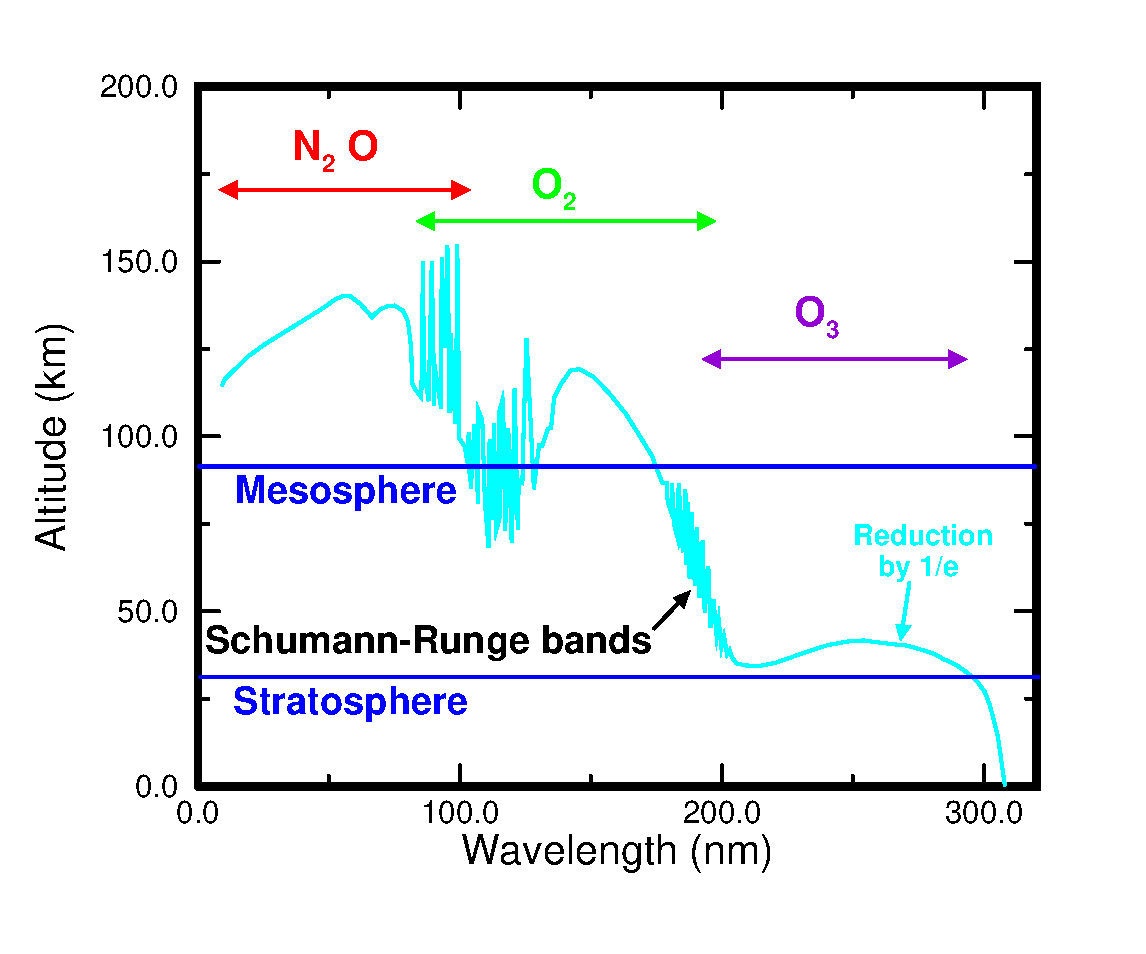
\includegraphics[width=10cm]{fig1.eps}
  \end{center}
\caption{This is an example of how to include an eps (encapsulated postscript) figure. Maths is OK in the caption $\epsilon^2 =\Delta$. }
\label{some text as a figure label}
\end{figure}
%
Notice how I can refer to the figure, Fig.~\ref{some text as a figure label}. 
